\documentclass{standalone}
\usepackage{tikz}
\usetikzlibrary{arrows.meta}
\renewcommand{\familydefault}{\sfdefault} % Sans serif

\begin{document}	
	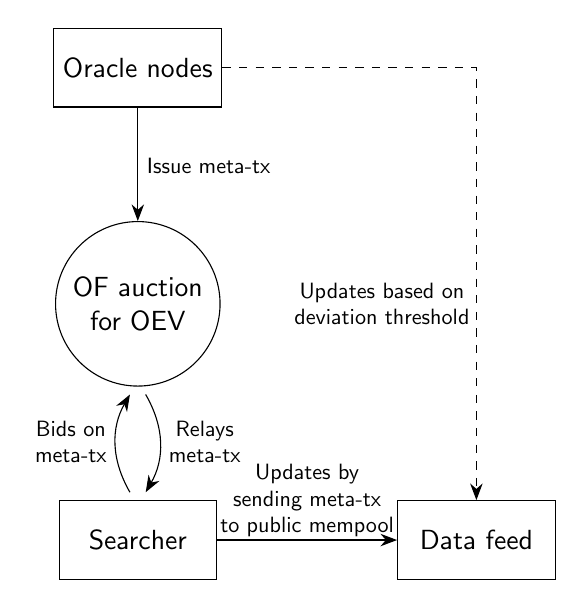
\begin{tikzpicture}
	\node[draw, circle, align=center, minimum size=2cm] at (0,0) (of-auction) {OF auction\\for OEV};
	\node[draw, align=center, minimum width=2cm,minimum height=1cm] at (0,3) (oracle-nodes) {Oracle nodes};
	\node[draw, align=center, minimum width=2cm,minimum height=1cm] at (0,-3) (searcher) {Searcher};
	\node[draw, align=center, minimum width=2cm,minimum height=1cm] at (4.3, -3) (data-feed) {Data feed};

	\draw[-{Stealth[scale=1.25]}] (oracle-nodes) to (of-auction);
	\node[align=center, scale=0.8] at (0.9, 1.75) {Issue meta-tx};

	\draw[-{Stealth[scale=1.25]}, bend left] ([shift={(-0.1,0.1)}]searcher.north) to ([shift={(-0.1,-0.1)}]of-auction.south);
	\draw[-{Stealth[scale=1.25]}, bend left] ([shift={(0.1,-0.1)}]of-auction.south) to ([shift={(0.1,0.1)}]searcher.north);
	\node[align=center, scale=0.8] at (0.85, -1.75) {Relays\\meta-tx};
	\node[align=center, scale=0.8] at (-0.85, -1.75) {Bids on\\meta-tx};
	
	\draw[-{Stealth[scale=1.25]}] (searcher) to (data-feed);
	\node[align=center, scale=0.8] at (2.15, -2.5) {Updates by\\sending meta-tx\\to public mempool};
	
	\draw[-{Stealth[scale=1.25]}, dashed] (oracle-nodes) to (4.3, 3) to (data-feed);
	\node[align=center, scale=0.8] at (3.1, 0) {Updates based on\\deviation threshold};
	\end{tikzpicture}
\end{document}